\section{Conclusion and Future Work}
\label{sec:conclusion}

The two-stage pipeline presented in this report demonstrates that physically plausible character animation from casual video is tractable within a unified adversarial-diffusion framework. ViMo-Flow generates kinematically coherent 3D motion from unconstrained footage via DDPM with Min-SNR reweighting and Probabilistic Timestep Sampling, without requiring explicit camera calibration. The physics-based imitation stage drives a MuJoCo humanoid to reproduce these kinematics under rigid-body dynamics through body-part-specific discriminators and PPO, eliminating hand-crafted reward engineering. Composite multi-objective reward aggregation and goal-conditioned extensions demonstrate that the adversarial reward paradigm scales to multi-skill learning beyond single-clip imitation.

Experiments across three locomotion difficulty tiers confirm that the baseline adversarial controller scales with motion complexity and that both auxiliary mechanisms studied---phase-conditioned observations and bilateral symmetry regularisation---offer narrow benefits on specific motion categories while introducing generalisation limitations that preclude their use as default components.

\paragraph{Limitations.}
The current simulation character is a 28-DOF ``humanoid-lite'' model: it collapses the SMPL skeleton's 24 joints and 72 axis-angle DOF into 15 rigid bodies to prioritise simulation stability. This simplification, motivated by the imitation-learning literature~\cite{deepmimic2018, iccgan2021}, yields controllable locomotion but fails on motions that demand simultaneous, coupled articulation of all major joints---high-energy dance steps, aerial phases, and skidding contact patterns all require joint torques and momentum transfers that the reduced model cannot faithfully reproduce.

A secondary limitation is dataset coverage. AIST++ provides choreographed single-person dance; retargeted clips retain the gross body trajectory but lose subtle upper-body articulation through chain-composition in the converter. ViMo-Flow outputs, while more diverse, carry kinematic errors from the diffusion inference that the discriminator cannot always absorb.

\paragraph{Planned Extensions.}

\begin{enumerate}
    \item \textbf{Extended humanoid (34 DOF).} The simulation character will be upgraded from the current DeepMimic 28-DOF body to a 34-DOF rig that mirrors the SMPL joint count more closely---restoring individual spine segments, collarbones, and hand articulations as actuated joints. This is expected to unlock complex dance motions where upper-body and lower-body coordination is non-trivial, at the cost of a harder learning problem requiring longer training and potentially curriculum initialisation.

    \item \textbf{Complex motion support.} With the richer character model, focus will shift to motions currently out of reach: jumps and landings (aerial impulse + contact recovery), lateral shuffles and pivots, and asymmetric arm-leg coordination seen in jaunty walk and dance genres. These require refining the retargeting pipeline to preserve aerial-phase root trajectories and extending the discriminator window to capture contact transitions over longer horizons.

    \item \textbf{Policy adaptation.} Once stable physics-based control is established on the extended character, the third stage of the pipeline---policy adaptation via AdaptNet~\cite{adaptnet2023}---will be integrated. The two-tier adaptation hierarchy (latent-embedding perturbation for modest shifts; deep-layer modification for substantial environment or morphology changes) addresses deployment robustness when the simulation parameters or task objectives differ from training conditions. This stage was deferred to ensure the base imitation policy is stable enough to serve as an initialisation point for adaptation.
\end{enumerate}


%%%%%%%%%%%%%%%%%%%%%%%%%%%%%%%%%%%%%%%%%%%%%%%%%%%%%%%%%%%%%%%%%%%%%
%\newpage
\vspace{5em}
\section{Results}
\label{sec:results}

\noindent\textit{ViMo-Flow qualitative samples for different vimo configurations and thier outputs are covered here: Appendix~\ref{sec:vimo_results} as part of previous study.}\par

\subsection{ICCGAN Humanoid Motions}

The adversarial imitation framework employs an ensemble of body-part-specific discriminators trained in tandem with a PPO policy. The discriminators distinguish reference mocap trajectories from policy-generated ones on subsets of joints (e.g., lower-body, upper-body, full-body), providing dense reward signals without manual tuning. The policy maximizes the probability of fooling these classifiers while satisfying dynamics constraints in the MuJoCo simulator. Default parameters (horizon \( H = 16 \), \( N = 32 \) environments, simulation rate 120\,Hz, learning rates \( 5 \times 10^{-6} \) actor / \( 10^{-4} \) critic / \( 10^{-5} \) discriminator) are used across runs, with configs overriding env-specific values such as \texttt{grace\_steps} for ground-contact motions.

Performance is quantified via lifetime cycles (fraction of maximum episode length survived), mean reward, discriminator gap (\( D_{\text{real}} - D_{\text{fake}} \)), and per-discriminator scores. Table~\ref{tab:iccgan_metrics} presents final-period statistics (epochs 19\,000--20\,000, averaged over logged intervals) extracted from training traces.

\begin{figure}[H]
    \centering
    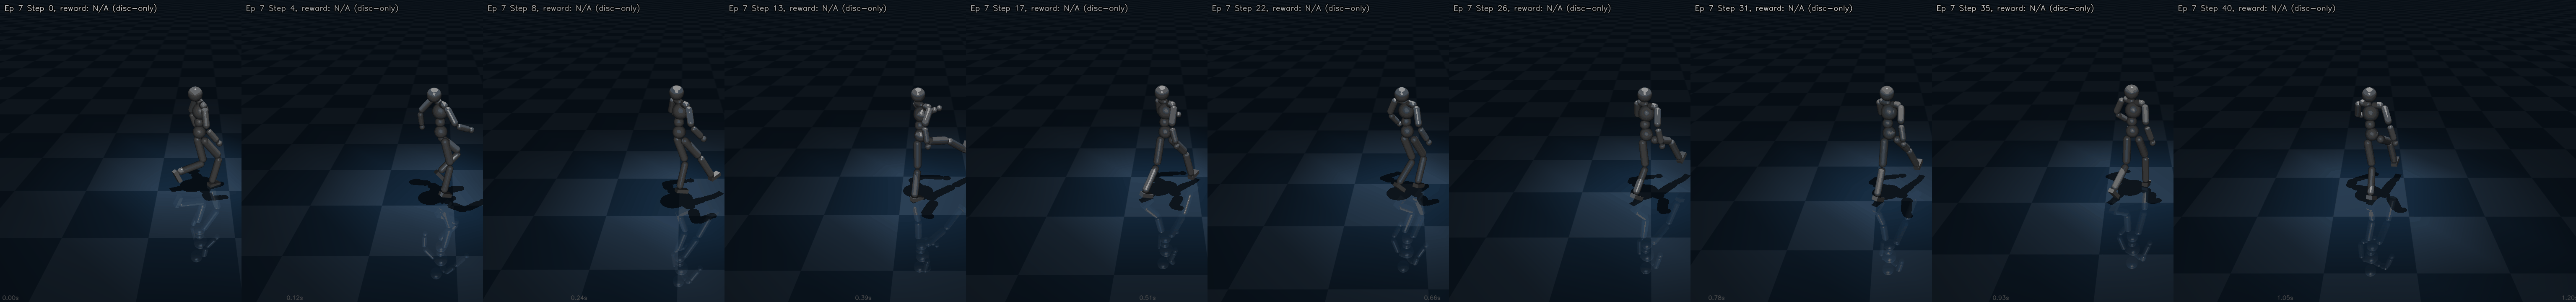
\includegraphics[width=\textwidth]{outputs/simulations/jaunty_walk.png}
    \caption{Jaunty walk}
    \label{fig:jaunty_sim}
\end{figure}

\begin{figure}[H]
    \centering
    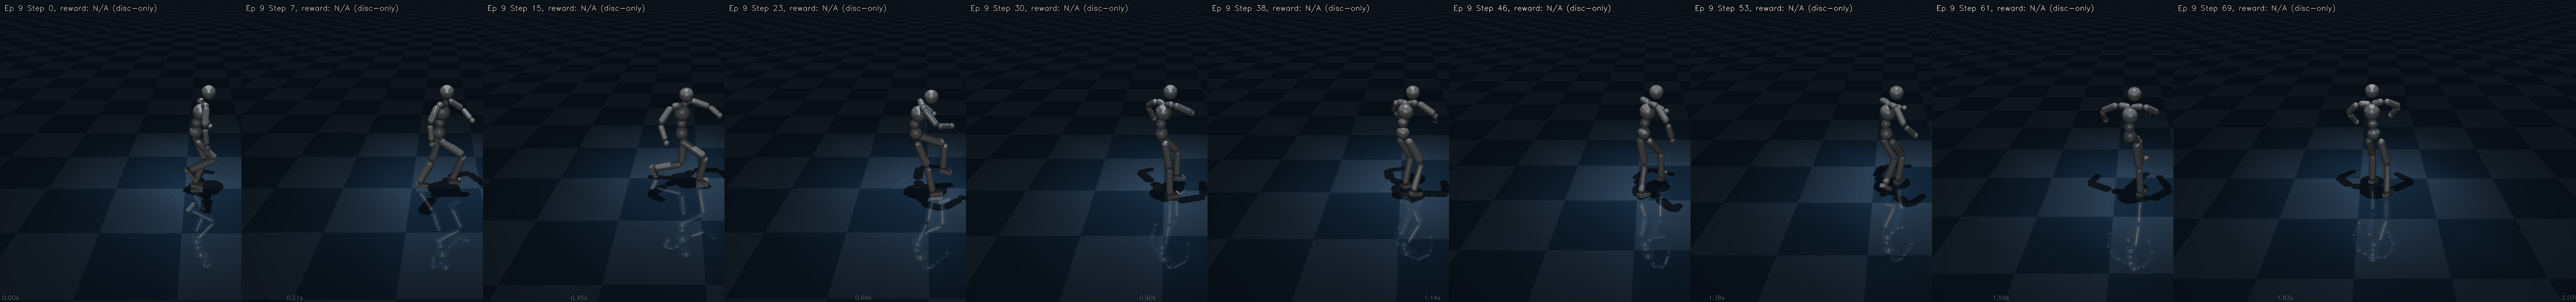
\includegraphics[width=\textwidth]{outputs/simulations/joyful_walk.png}
    \caption{Joyful walk}
    \label{fig:joyful_sim}
\end{figure}

\begin{figure}[H]
    \centering
    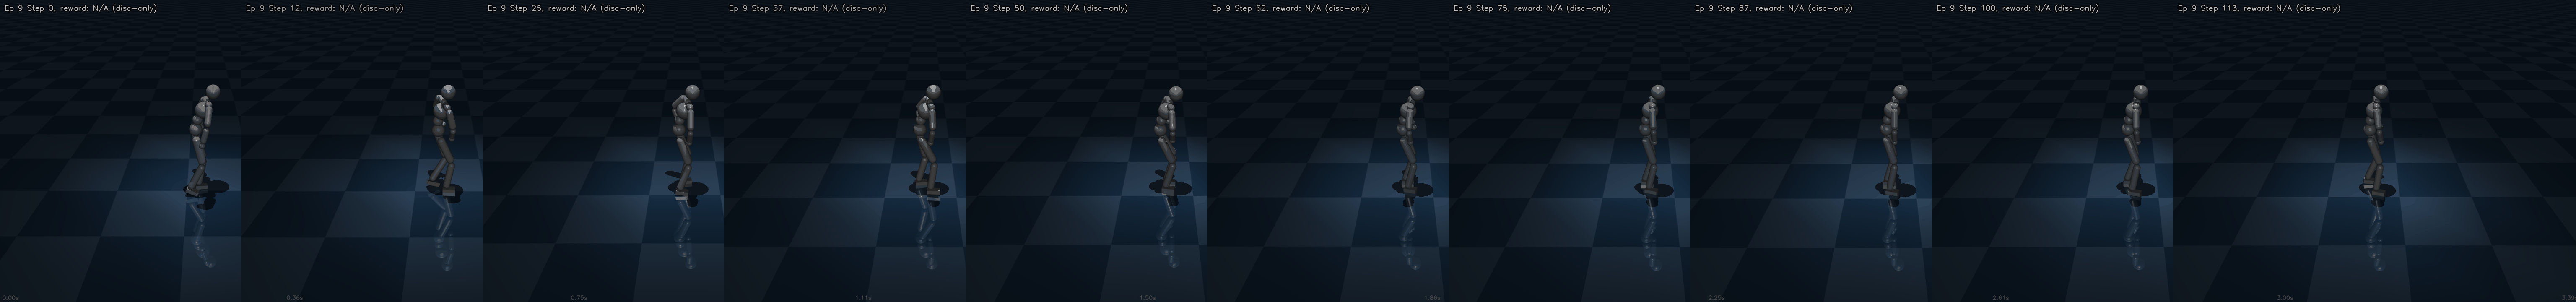
\includegraphics[width=\textwidth]{outputs/simulations/limp_walk.png}
    \caption{Limp walk}
    \label{fig:limp_sim}
\end{figure}

\begin{table}[htbp]
\centering
\caption{ICCGAN motion imitation performance at convergence (Period 20). Highlights used to substantiate inferences on replication fidelity, stability, and termination behavior.}
\label{tab:iccgan_metrics}
\resizebox{\textwidth}{!}{
\begin{tabular}{lccccccc}
\toprule
Motion & Lifetime Cycles & Reward Mean & Disc. Gap & Score Real & Score Fake & Steps & Inference Highlight \\
\midrule
squat     & 0.4948 $\pm$ 0.0510 & 0.1938 $\pm$ 0.0289 & 0.5399 & 0.7321 & 0.1922 & 84 & perfect replication (fixed leg pose) \\
punch     & 0.5051 $\pm$ 0.0650 & 0.3694 $\pm$ 0.0258 & 0.4123 & 0.7823 & 0.3700 & 39 & highest survival/reward; minor leg slip \\
leg\_lunge & 0.4923 $\pm$ 0.0515 & 0.3281 $\pm$ 0.0367 & 0.3919 & 0.7185 & 0.3266 & 109 & high cycles but value-loss variance indicates slipperiness \\
kick      & 0.3942 $\pm$ 0.0672 & 0.1481 $\pm$ 0.0235 & 0.3641 & 0.5248 & 0.1607 & 56 & moderate survival; hip-range instability causes falls \\
long\_jump & 0.3639 $\pm$ 0.0620 & 0.0754 $\pm$ 0.0226 & 0.3483 & 0.4451 & 0.0968 & 53 & improved landing at moderate run speed \\
roll      & 0.0575 $\pm$ 0.0095 & -0.1367 $\pm$ 0.0125 & 0.1978 & 0.1700 & -0.0278 & 99 & critically low cycles despite \texttt{grace\_steps}; termination hurdle \\
\bottomrule
\end{tabular}}
\end{table}

\begin{figure}[htbp]
\centering
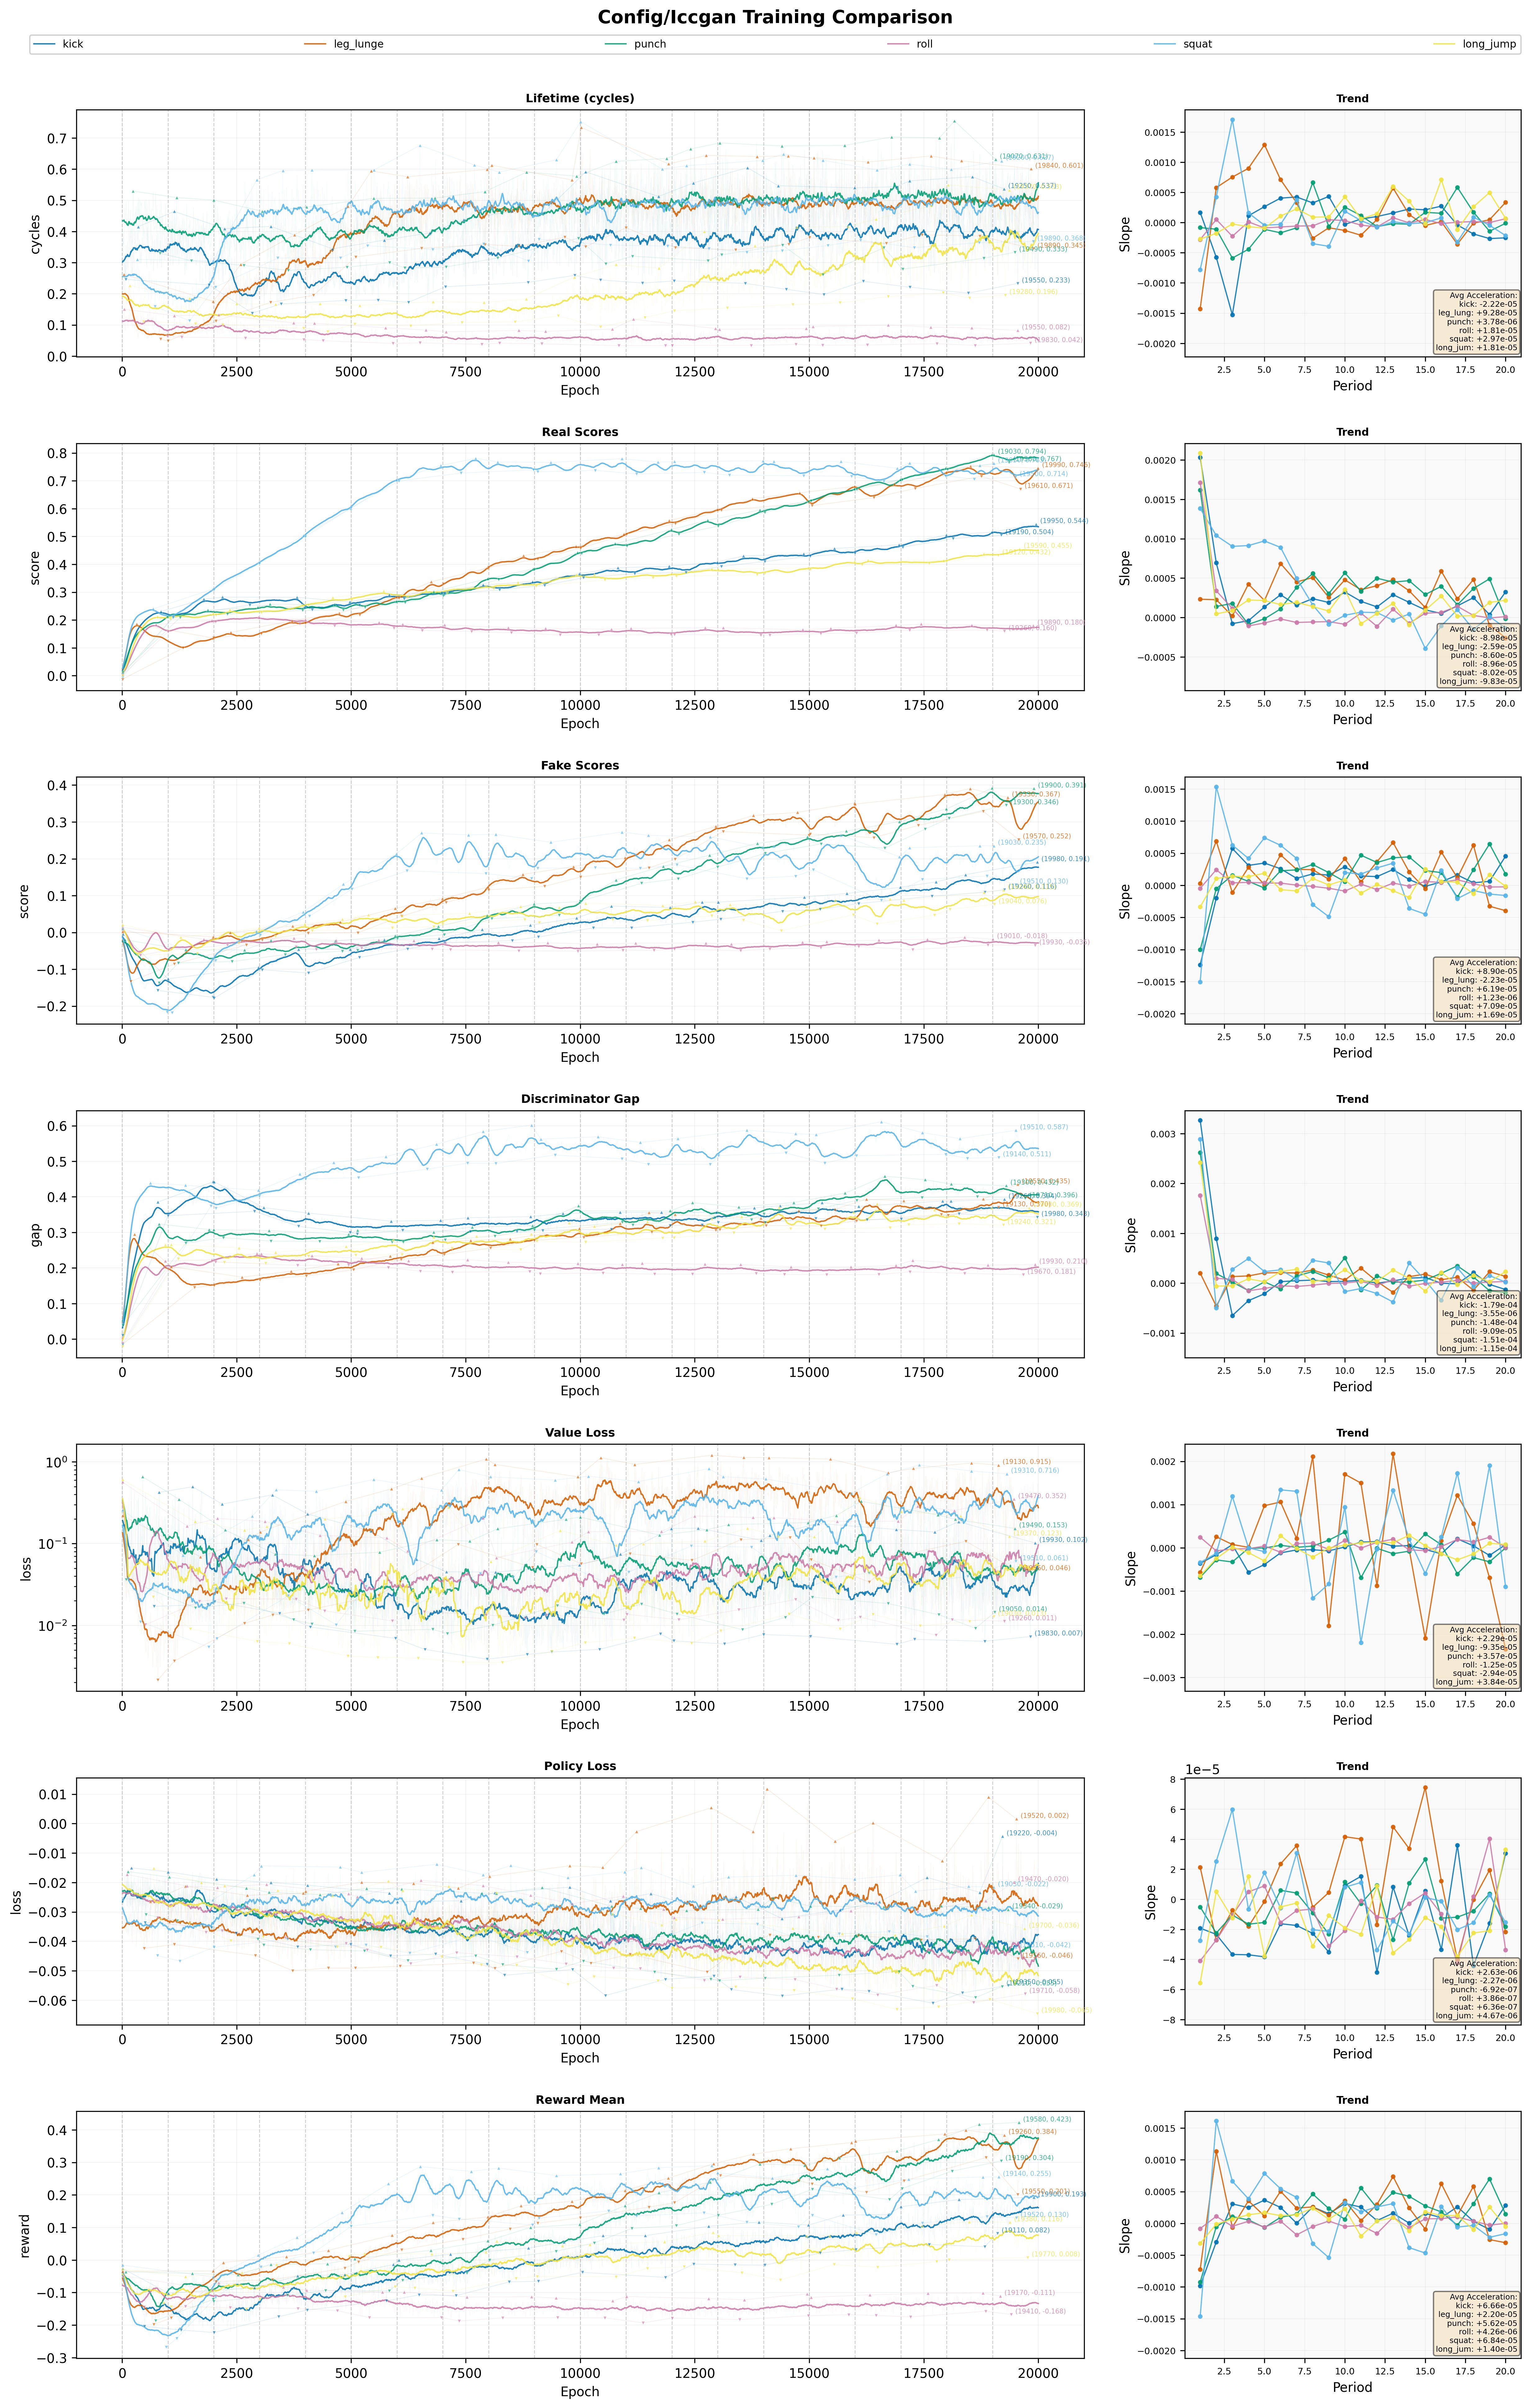
\includegraphics[height=.925\textheight, keepaspectratio]{outputs/case_studies/iccgan_comparison.png}
\caption{Comparative training curves across ICCGAN motions}
\label{fig:iccgan_comparison}
\end{figure}

\begin{figure}[H]
    \centering
    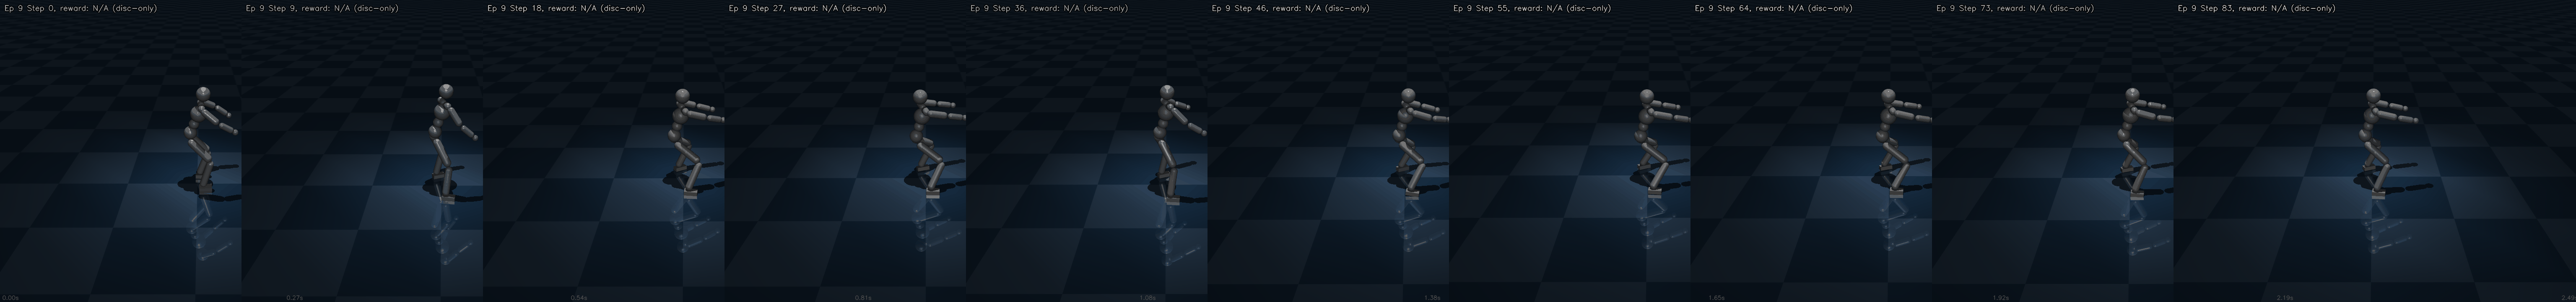
\includegraphics[width=\textwidth]{outputs/simulations/squat.png}
    \caption{Squat -- stable pose with legs fixed, zero slip observed}
    \label{fig:squat_sim}
\end{figure}

\textbf{Squat.} Perfect kinematic and dynamic replication is attained. The motion constrains leg joints to near-constant positions, eliminating balance challenges. This is numerically corroborated by the highest stable lifetime cycles (0.49 of maximum), consistently positive reward (0.1938), and strong real discriminator score (0.732). Simulation frames (Figure~\ref{fig:squat_sim}) confirm exact pose matching without drift; the humanoid maintains the crouched configuration throughout the episode without CoM excursions.

\begin{figure}[H]
    \centering
    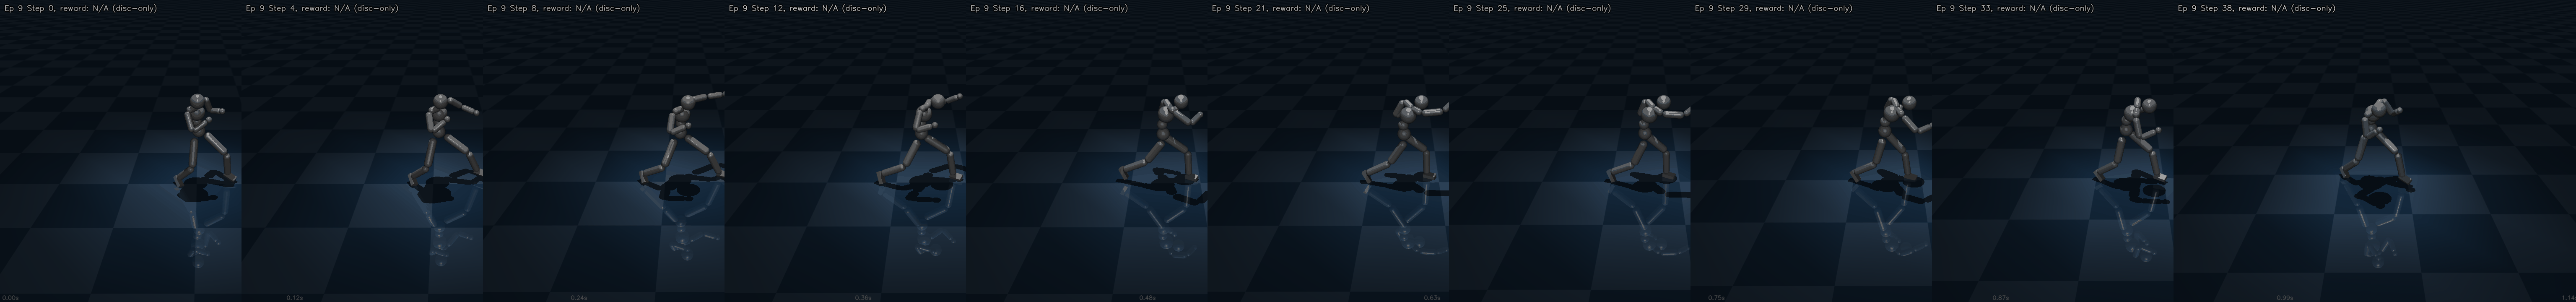
\includegraphics[width=\textwidth]{outputs/simulations/punch.png}
    \caption{Punch -- upper-body dominant action with minor terminal leg slippage}
    \label{fig:punch_sim}
\end{figure}

\textbf{Punch and leg lunge.} Near-perfect imitation with only minor leg slipperiness in terminal phases. Both achieve top-tier survival (0.51 and 0.49 cycles) and reward (0.37 and 0.33), with score\_fake approaching real (0.37 and 0.33). The slight slippage manifests as elevated value-loss variance in lunge (0.31) but does not compromise overall stability, validating the discriminator ensemble's efficacy for upper-body dominant actions. Figure~\ref{fig:punch_sim} illustrates the forward thrust with stable base; lunge exhibits analogous behavior with minor foot repositioning at motion end.

\begin{figure}[H]
    \centering
    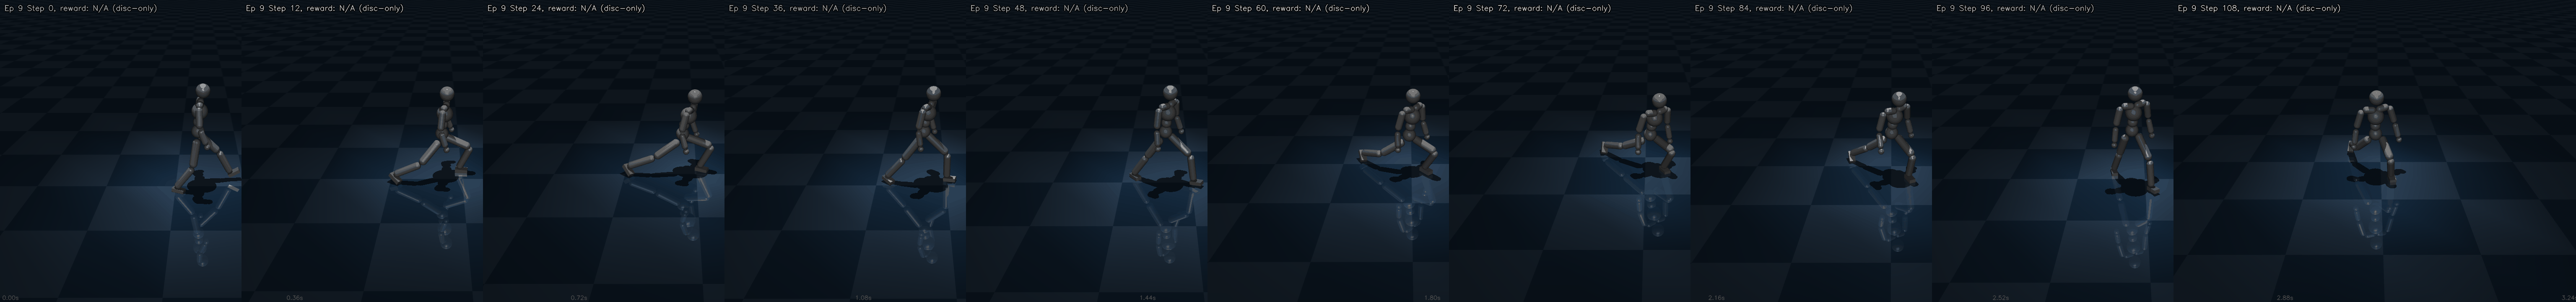
\includegraphics[width=\textwidth]{outputs/simulations/leg_lunge.png}
    \caption{Leg lunge -- controlled forward extension with minor slip at terminal phase}
    \label{fig:lunge_sim}
\end{figure}

\textbf{Leg lunge.} The policy achieves high-cycle performance (0.49) with strong reward (0.328), though value-loss variance (0.31) indicates intermittent foot slip during the extension phase. Figure~\ref{fig:lunge_sim} visualizes the controlled forward step; the slight repositioning at motion conclusion accounts for the variance without destabilizing the overall trajectory.

\begin{figure}[H]
    \centering
    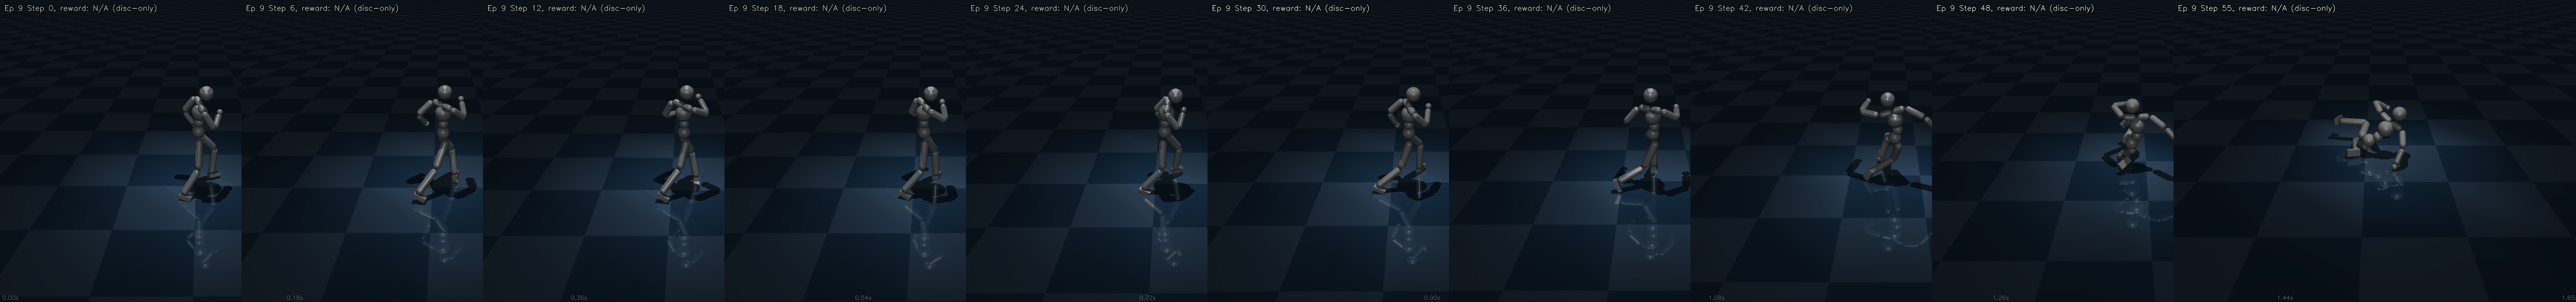
\includegraphics[width=\textwidth]{outputs/simulations/kick.png}
    \caption{Kick -- hip-driven swing with support leg instability leading to falls}
    \label{fig:kick_sim}
\end{figure}

\textbf{Kick.} The policy initiates the hip-driven swing but frequently loses balance on the support leg, leading to falls before completion. Lifetime cycles plateau at 0.39 with reward 0.148; episodes terminate prematurely when center-of-mass projection exits the support polygon. Occasional successful kicks occur but cannot maintain one-legged stance, as evidenced by the moderate score\_real (0.52) compared to squat/punch. Figure~\ref{fig:kick_sim} captures the initiation phase; subsequent frames show the characteristic collapse when weight shifts to the planted foot.

\begin{figure}[H]
    \centering
    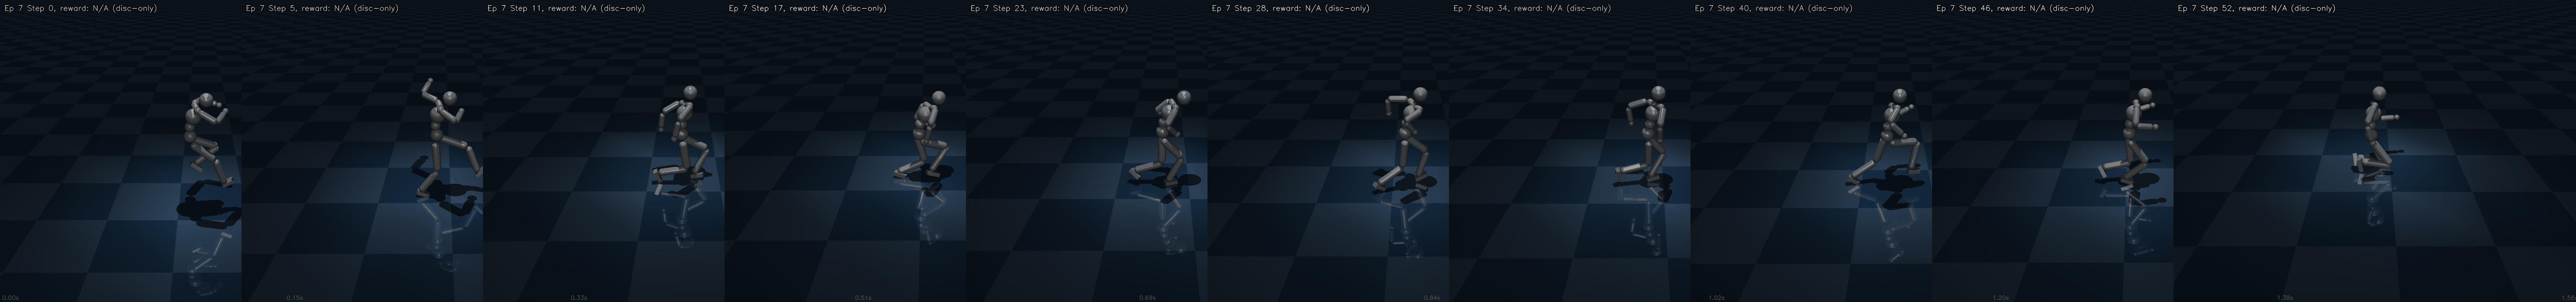
\includegraphics[width=\textwidth]{outputs/simulations/long_jump.png}
    \caption{Long jump -- takeoff and landing phases with speed-dependent stability}
    \label{fig:longjump_sim}
\end{figure}

\textbf{Long jump.} Landing fidelity improves markedly in episodes where takeoff run velocity remains moderate. Excessive forward lean during run-up (to counteract anticipated fall) produces compensatory acceleration, degrading landing stability. The 0.36 cycles and 0.075 reward reflect this sensitivity; renders in Figure~\ref{fig:longjump_sim} demonstrate successful cases under controlled speed. Episodes 4--6 in the checkpoint RGB arrays show clean landings when run speed is normal-paced; higher velocities introduce forward momentum that disrupts touchdown.

\begin{figure}[H]
    \centering
    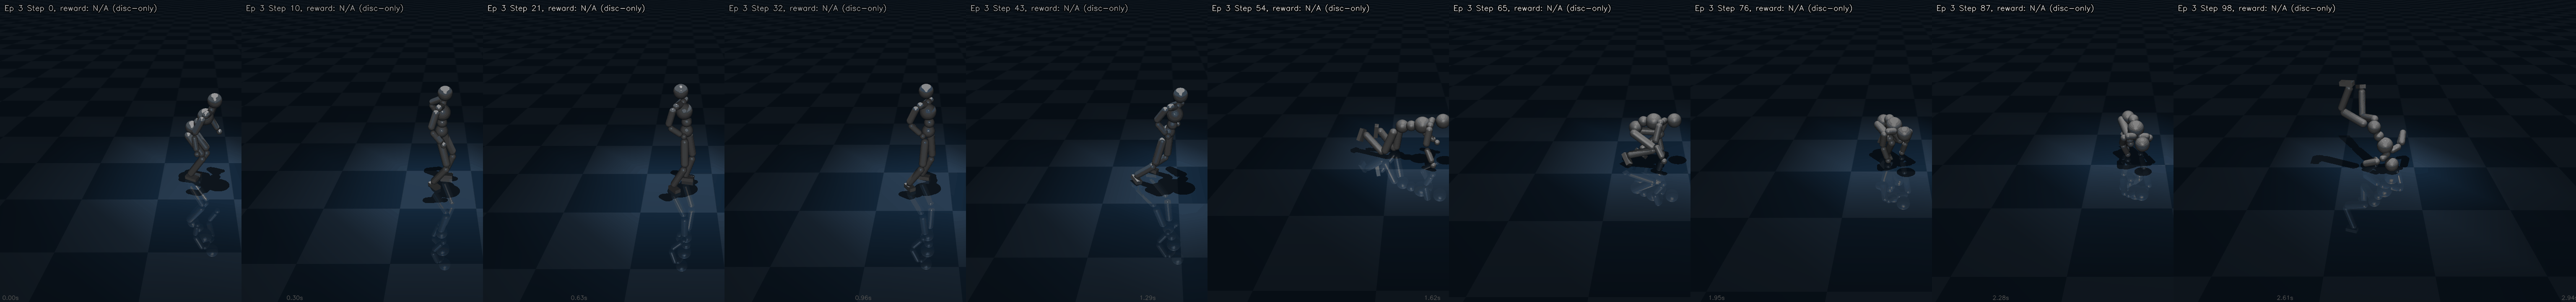
\includegraphics[width=\textwidth]{outputs/simulations/roll.png}
    \caption{Roll -- diving initiation captured; episode terminates upon ground contact (pelvis < 0.15m) preventing full recovery}
    \label{fig:roll_sim}
\end{figure}

\textbf{Roll.} Complete failure to complete the sequence despite targeted mitigation. The pelvis-height termination (<0.15\,m) triggers episode end precisely when the motion requires floor contact. The \texttt{grace\_steps} counter (extended in config) delays reset during prone states, allowing partial diving imitation, yet the policy cannot recover upright posture from fallen initial states. This is quantitatively confirmed by lifetime cycles collapsing to 0.0575, persistently negative reward (-0.137), and lowest scores. Figure~\ref{fig:roll_sim} captures the initial dive; the subsequent ground contact triggers termination before the rollover and upright recovery can execute. The implementation reveals a fundamental simulator limitation for motions violating the termination heuristic, addressed partially but insufficiently for full rollout recovery.

These results demonstrate that the body-part discriminator approach scales effectively to simple static and cyclic motions (squat, punch) but exposes limits on high-momentum asymmetric or ground-interaction behaviors (kick, roll). Overlapping frame composites and per-episode RGB arrays provide visual confirmation, with training curves showing rapid convergence for high-fidelity cases within 5\,000--10\,000 epochs.

The locomotion baselines (jaunty, joyful, limp walks) were analyzed in the experimental section; the above extends the evaluation to a broader mocap suite, confirming the pipeline's adaptability for mocap-driven physics-based animation while highlighting directions for extended DOF models and refined termination logic.

\subsection{Vimo Full-Body Dance Motions (AIST Retargeted)}

ViMo-generated full-body dance sequences from the AIST Dance Video Database were retargeted and grouped by \texttt{dance\_genre/choreography\_id}. Per the AIST naming convention (\texttt{gXX\_sBM\_cAll\_dXX\_mXX\_chYY}), the choreography ID defines the core sequence while musical piece IDs vary tempo. Motions sharing the same choreography ID are structurally similar with only execution speed differences. Grouping enables a single policy to learn from a family of related references, improving generalization across tempo variations. Movement descriptions derive from frame-wise comparison images in the preview assets.

\begin{table}[htbp]
\centering
\caption{Vimo dance motion performance at convergence (Period 30). Numerical highlights from training traces directly substantiate inferences on stability, converter artifacts, and partial success.}
\label{tab:vimo_metrics}
\resizebox{\textwidth}{!}{
\begin{tabular}{lccccccc}
\toprule
Motion & Lifetime Cycles & Reward & Disc Gap & Score Real & Score Fake & Steps & Inference Highlight \\
\midrule
gBR/ch01 (indian step) & 0.20 $\pm$0.04 & 0.079 $\pm$0.016 & 0.484 & 0.569 & 0.085 & 304 & side-step falls; limited recovery \\
gHO/ch01 (loose legs) & 0.36 $\pm$0.05 & 0.176 $\pm$0.014 & 0.526 & 0.702 & 0.175 & 240 & sliding legs cause balance loss \\
gJS/ch02 (pos. des pieds) & 0.02 $\pm$0.00 & -0.182 $\pm$0.007 & 0.304 & 0.179 & -0.125 & 281 & foot clipping from SMPL$\to$28DOF converter causes collapse \\
gLH/ch01 (slide) & 0.35 $\pm$0.06 & 0.136 $\pm$0.017 & 0.531 & 0.667 & 0.136 & 322 & partial success; tempo-induced hand instability \\
gLO/ch02 (twirl) & 0.48 $\pm$0.04 & 0.096 $\pm$0.010 & 0.463 & 0.557 & 0.094 & 276 & high survival but nullifies rhythmic knee bends \\
gMH/ch02 (rock board) & 0.24 $\pm$0.04 & 0.093 $\pm$0.018 & 0.524 & 0.621 & 0.097 & 293 & complete failure on leg-lift instability \\
gPO/ch01 (fresno) & 0.47 $\pm$0.05 & 0.205 $\pm$0.057 & 0.453 & 0.659 & 0.206 & 306 & legs prioritize stability; arms mimic reference \\
\bottomrule
\end{tabular}}
\end{table}

\begin{figure}[htbp]
\centering
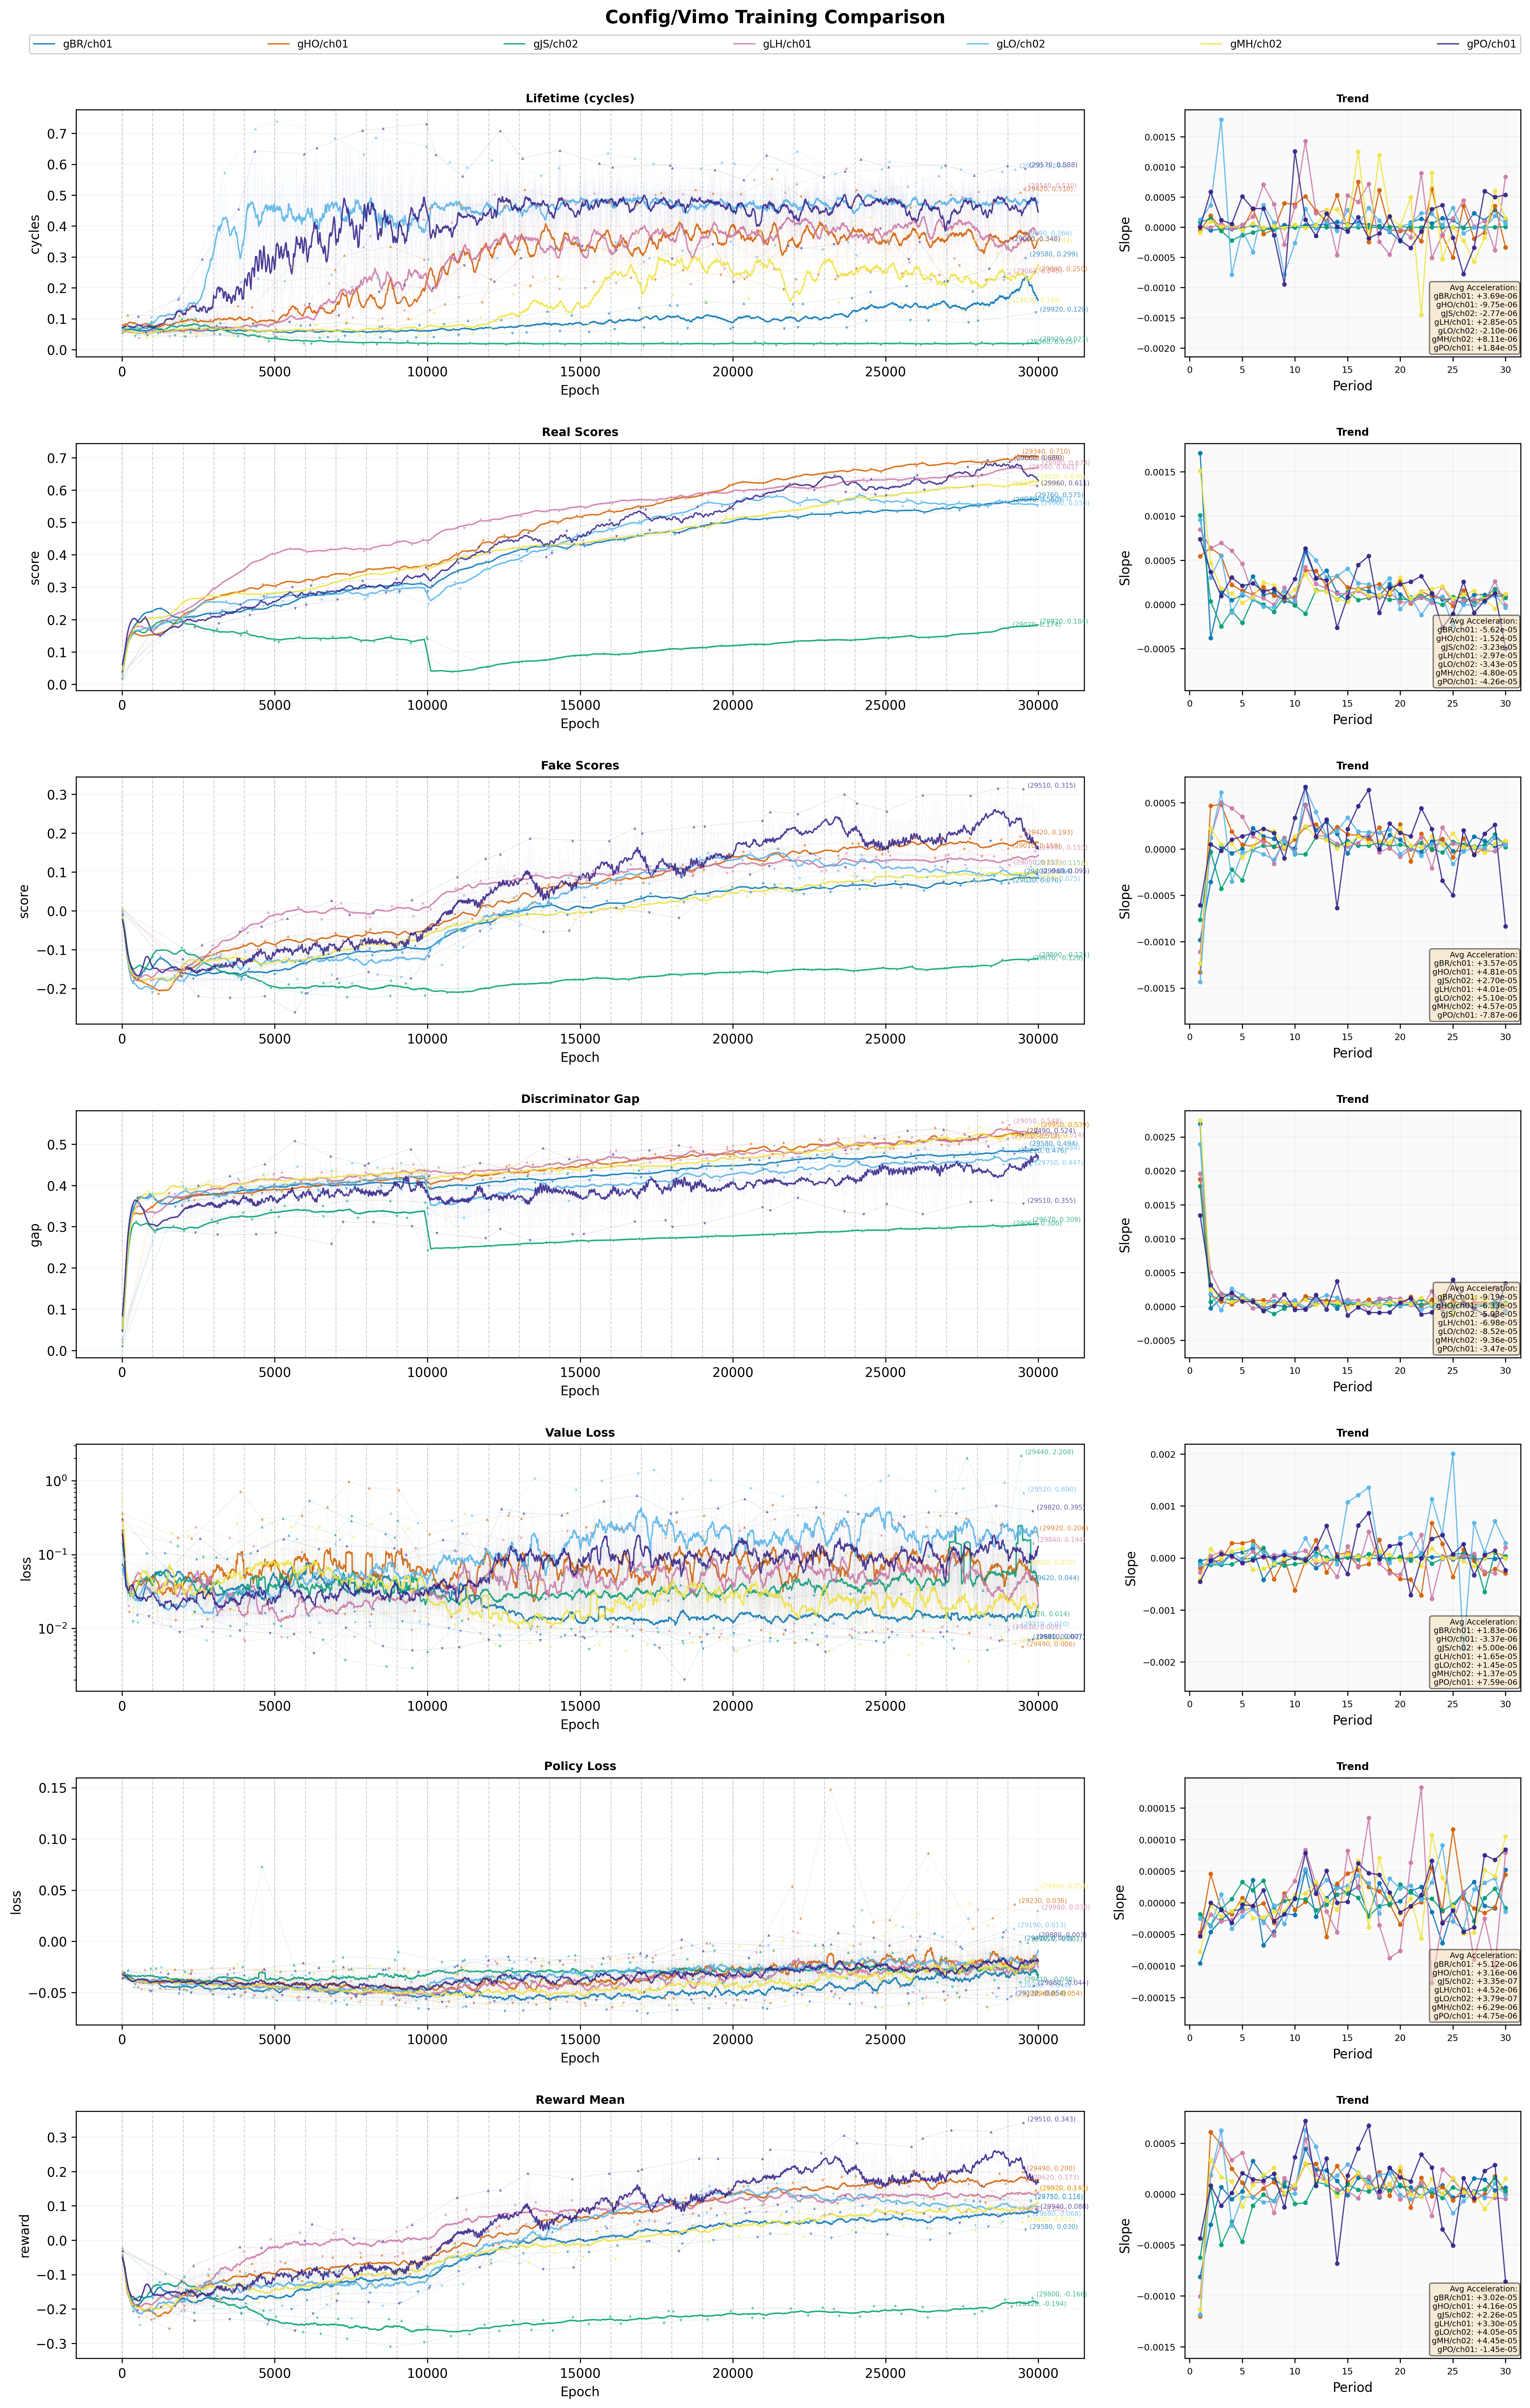
\includegraphics[height=.925\textheight, keepaspectratio]{outputs/case_studies/vimo_comparison.png}
\caption{Vimo training curves across dance genres.}
\label{fig:vimo_comparison}
\end{figure}


\begin{figure}[H]
    \centering
    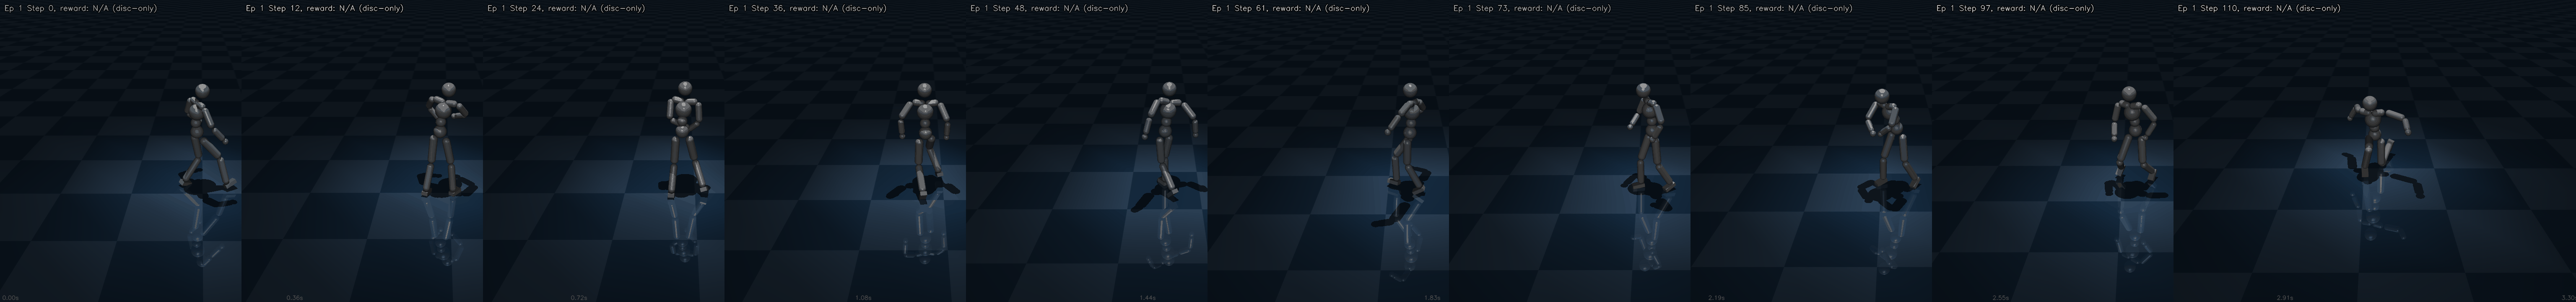
\includegraphics[width=\textwidth]{outputs/simulations/gBR_ch01.png}
    \caption{gBR/ch01 side-step falls}
    \label{fig:gbr_sim}
\end{figure}

\begin{figure}[H]
    \centering
    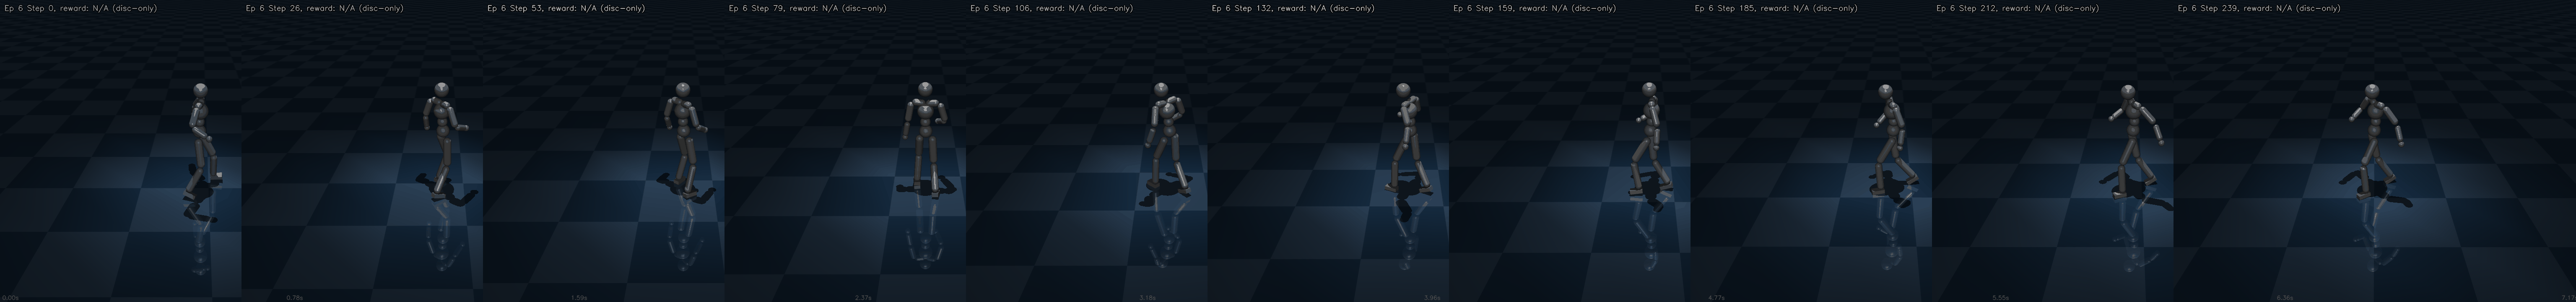
\includegraphics[width=\textwidth]{outputs/simulations/gHO_ch01.png}
    \caption{gHO/ch01 sliding legs}
    \label{fig:gho_sim}
\end{figure}

\textbf{gBR/ch01.} Side-step movements cause falls. Few balancing episodes fail to follow the subsequent dance step (lifetime 0.20 cycles, reward 0.079; Figure~\ref{fig:gbr_sim}).

\textbf{gHO/ch01.} Sliding leg motions lead to balance loss. Controller struggles with solid foot plants (lifetime 0.36, reward 0.176; Figure~\ref{fig:gho_sim}).

\begin{figure}[h]
    \centering
    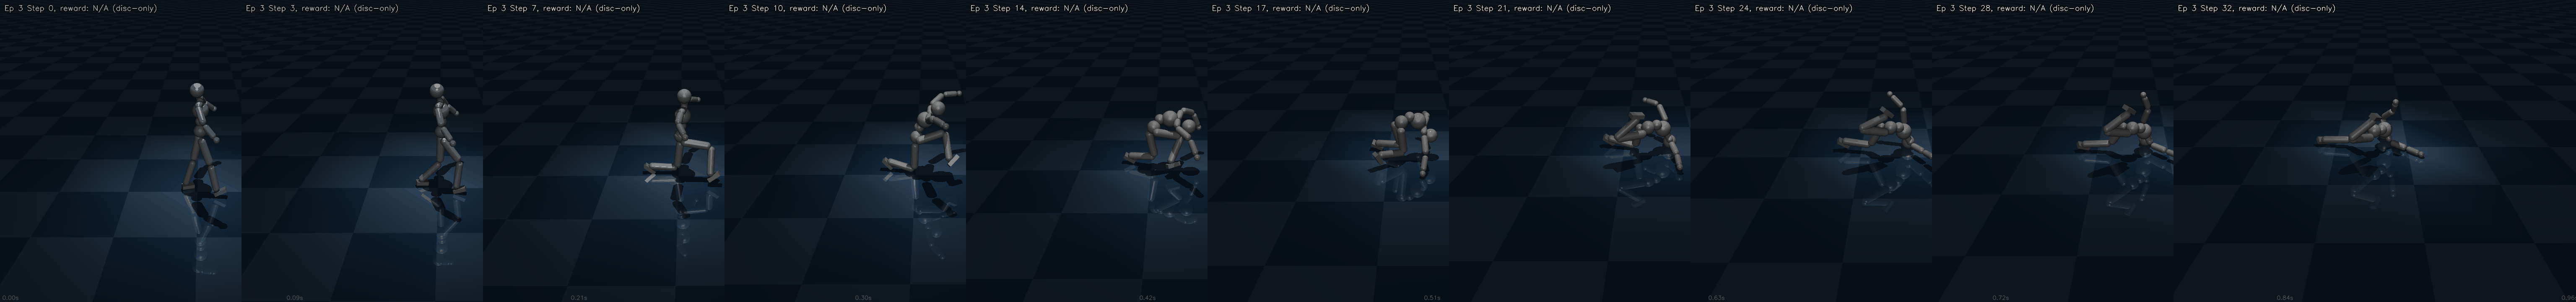
\includegraphics[width=\textwidth]{outputs/simulations/gJS_ch02.png}
    \caption{gJS/ch02 foot clipping collapse}
    \label{fig:gjs_sim}
\end{figure}

\begin{figure}[H]
    \centering
    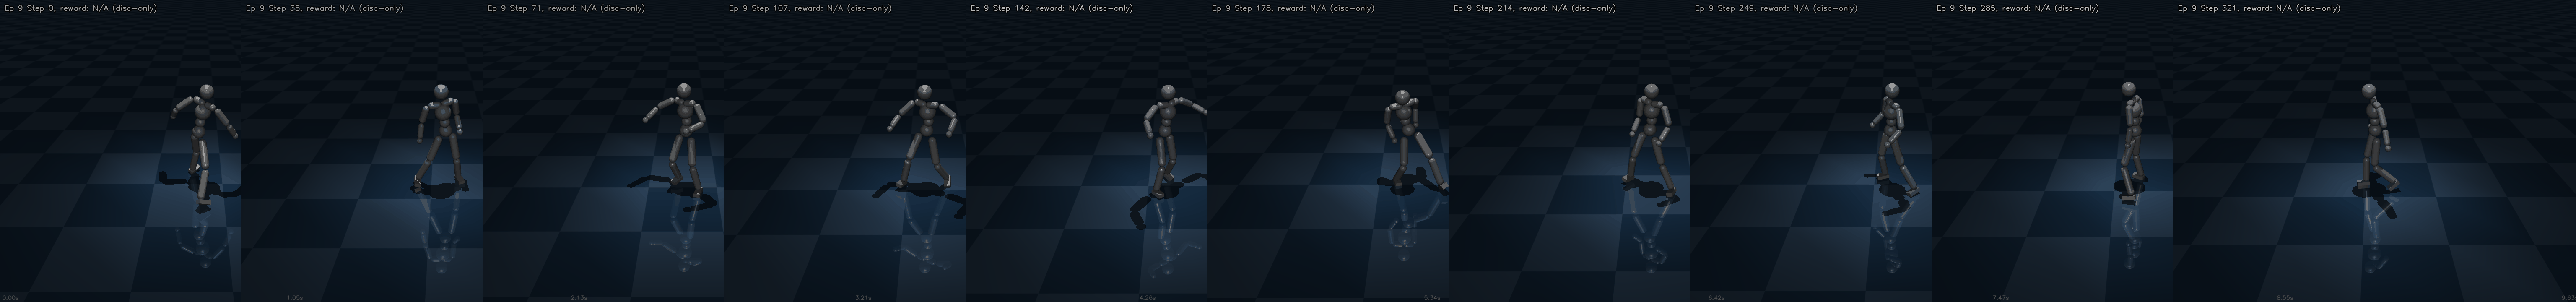
\includegraphics[width=\textwidth]{outputs/simulations/gLH_ch01.png}
    \caption{gLH/ch01 partial slide success}
    \label{fig:glh_sim}
\end{figure}

\textbf{gJS/ch02.} Easiest motion yet yields near-zero lifetime (0.02 cycles) and negative reward (-0.182). Reference feet clip into floor due to SMPL-to-28DOF converter (ankle+toe averaged into single joint). This induces physics collapse (Figure~\ref{fig:gjs_sim}).

\textbf{gLH/ch01.} Simpler sliding dance. Controller produces reduced sliding with higher-tempo hands causing instability. Partial success (0.35 cycles, 0.136 reward, real score 0.667; Figure~\ref{fig:glh_sim}).

\begin{figure}[H]
    \centering
    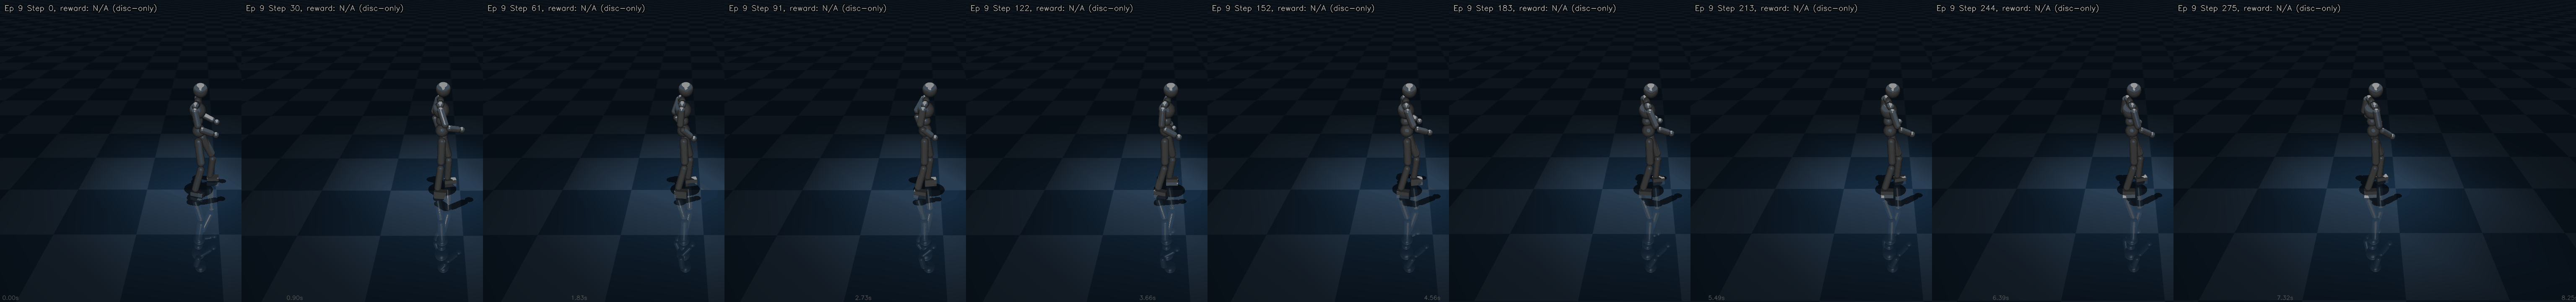
\includegraphics[width=\textwidth]{outputs/simulations/gLO_ch02.png}
    \caption{gLO/ch02 stabilization over knee bends}
    \label{fig:glo_sim}
\end{figure}

\begin{figure}[H]
    \centering
    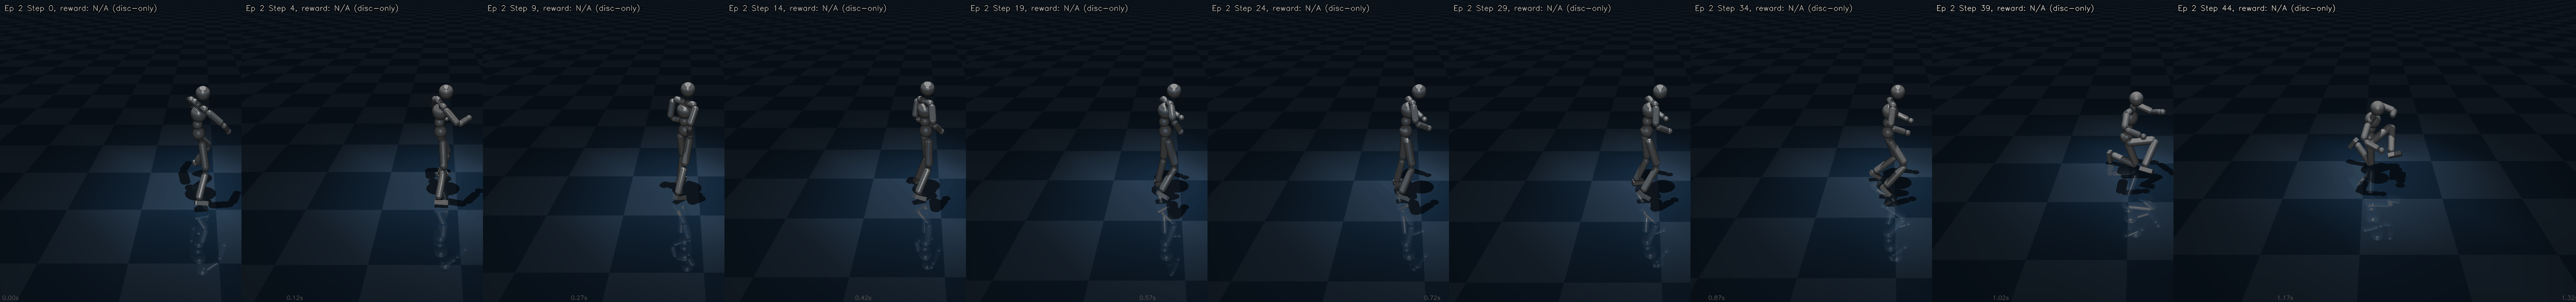
\includegraphics[width=\textwidth]{outputs/simulations/gMH_ch02.png}
    \caption{gMH/ch02 leg-lift failure}
    \label{fig:gmh_sim}
\end{figure}

\textbf{gLO/ch02.} Features abrupt freezes; selected clip is slow. Policy fails rhythmic knee bending, prioritizing stabilization (lifetime 0.48 but reward 0.096; Figure~\ref{fig:glo_sim}).

\textbf{gMH/ch02.} Leg lifts with bent support leg cause complete failure (lifetime 0.24, reward 0.093; Figure~\ref{fig:gmh_sim}).

\begin{figure}[H]
    \centering
    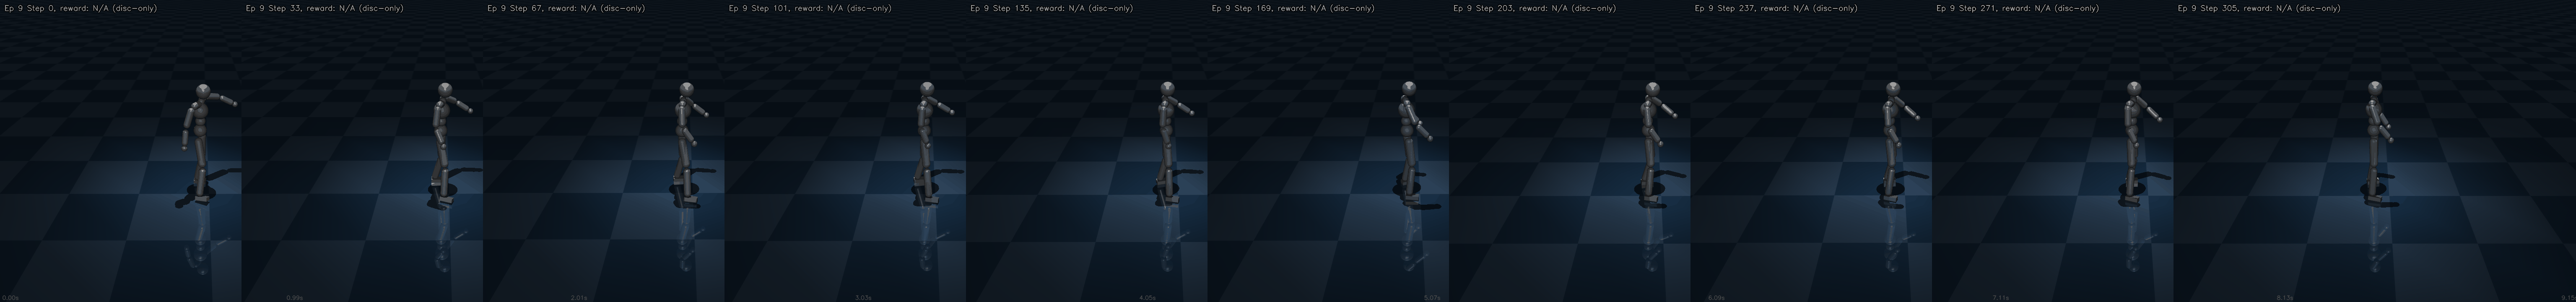
\includegraphics[width=\textwidth]{outputs/simulations/gPO_ch01.png}
    \caption{gPO/ch01 legs focus on stability}
    \label{fig:gpo_sim}
\end{figure}

\textbf{gPO/ch01.} Smooth genre; easy clip yields highest reward (0.205). Legs struggle for stability while hands better follow reference (lifetime 0.47 cycles; Figure~\ref{fig:gpo_sim}).

These Vimo evaluations, combined with ICCGAN results, confirm the adversarial framework's strengths on simpler gestures while exposing limits of the reduced-DOF model and retargeting on complex rhythmic dance. Numerical metrics from the final training period and side-by-side simulation frames guide refinement of the physics-based imitation pipeline toward real-world character animation automation.

\subsection{Task-Based Locomotion Simulations (LaFAN1)}

This category extends the imitation backbone with goal-directed control. Reference motions are drawn from the LaFAN1 dataset, grouping clips of \textit{walk}, \textit{run}, and \textit{crouched walk} with diverse starting positions and orientations. The grouped reference set enables the policy to imitate locomotion regardless of initial pose, while a task-specific reward steers the character toward an externally specified goal.

\paragraph{Task environment setup.}
Two task formulations are implemented; a third (Aiming) is implemented but not evaluated here.

\textit{Target Heading.} The character must move along a randomly sampled unit direction $\mathbf{g}_t \in \mathbb{R}^2$ resampled every 30 frames. The goal-directed reward measures alignment between the horizontal root displacement and the target heading:
\[
    r_t^G = \langle \dot{\mathbf{x}}^{\text{root}}_{t+1} / \|\dot{\mathbf{x}}_t\|, \, \mathbf{g}_t \rangle.
\]

\textit{Target Location.} The character must reach a goal position $\mathbf{p}^{\text{goal}}$ at a preferred speed. The reward is
\[
    r_t^G = \begin{cases} \exp\!\left(-3 \,\| \dot{\mathbf{x}}^{\text{root}}_{t+1}/\Delta t - \mathbf{v}^{\star}_t \|^2 / \|\mathbf{v}^{\star}_t\|^2 \right) & \text{if } \|\mathbf{x}_{t+1} - \mathbf{p}^{\text{goal}}\| > \rho \\ 1 & \text{otherwise}, \end{cases}
\]
with goal radius $\rho = 0.5$, sampling preferred speed in $[1, 1.5]\,m/s$ for walk/crouch and $[1, 3]\,m/s$ for run, with random direction in $[0, 2\pi)$ and timer in $[3,5]\,s$ (or $[2,3]\,s$ for run). The goal state $\mathbf{g}_t \in \mathbb{R}^4$ encodes direction unit vector, distance to goal, and preferred speed.

\textit{Aiming (implemented, untested).} A target aiming direction is encoded via the right-forearm orientation $\mathbf{d}^{\text{forearm}}_t$, with reward $r_t^G = \exp(-2\|\mathbf{d}^{\text{forearm}}_t - \mathbf{g}_t\|^2)$ when activated; otherwise an arm-lift bias keeps the gun raised.

\begin{table}[htbp]
\centering
\caption{Task-based locomotion performance at convergence.}
\label{tab:loco_metrics}
\resizebox{\textwidth}{!}{
\begin{tabular}{lccccccccc}
\toprule
Motion & Lifetime Cycles & Reward & Disc Gap & Score Real & Score Fake & Task Reward & Steps & Inference Highlight \\
\midrule
locomotion\_walk   & 0.31 $\pm$0.05 & 0.163 $\pm$0.065 & 0.413 & 0.694 & 0.281 & 0.170 $\pm$0.040 & 1253 & decent mimicry; struggles for wide deviation turns \\
locomotion\_run    & 0.27 $\pm$0.07 & -0.079 $\pm$0.084 & 0.535 & 0.585 & 0.050 & 0.078 $\pm$0.020 & 2122 & kangaroo-like hopping; partial mimicry despite longest training \\
locomotion\_crouch & 0.39 $\pm$0.05 & 0.064 $\pm$0.058 & 0.508 & 0.625 & 0.116 & 0.122 $\pm$0.031 & 666  & longest survival; train-wheel leg drag hack stabilizes turns \\
\bottomrule
\end{tabular}}
\end{table}

\begin{figure}[htbp]
    \centering
    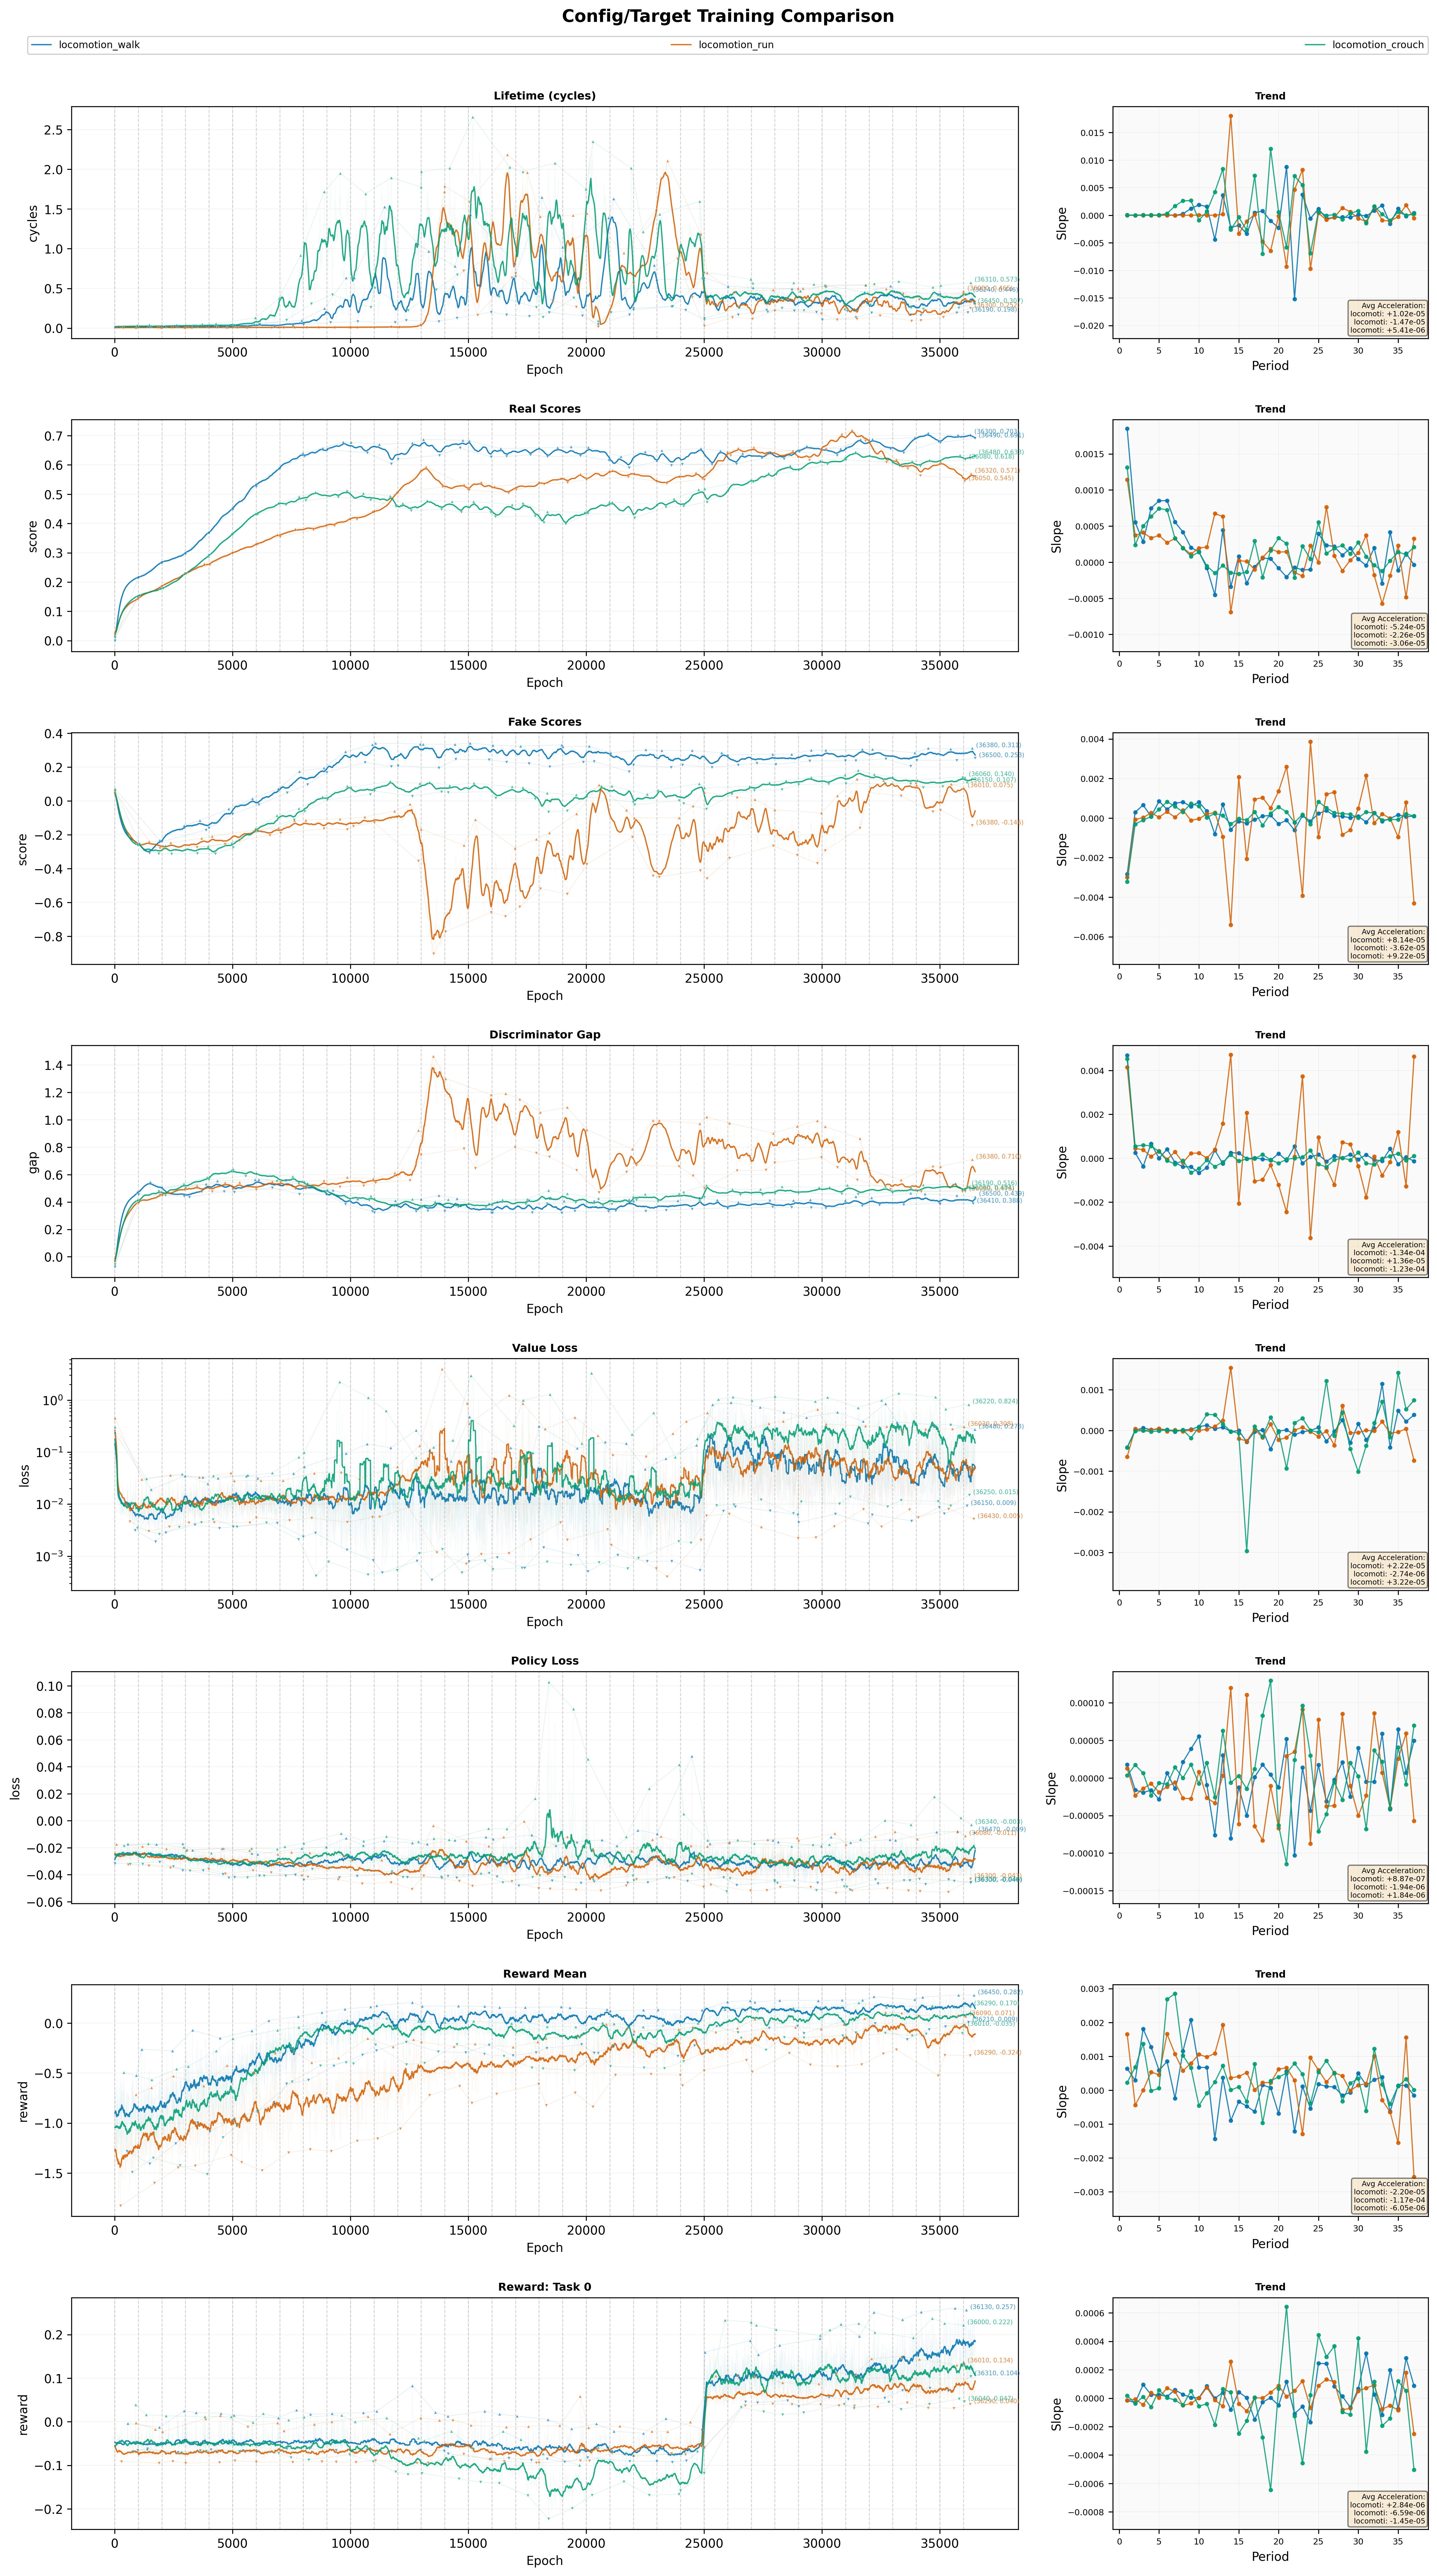
\includegraphics[height=.925\textheight, keepaspectratio]{outputs/case_studies/loco_comparison.png}
    \caption{Task-based locomotion training curves across walk, run, and crouch policies.}
    \label{fig:loco_comparison}
\end{figure}

\begin{figure}[H]
    \centering
    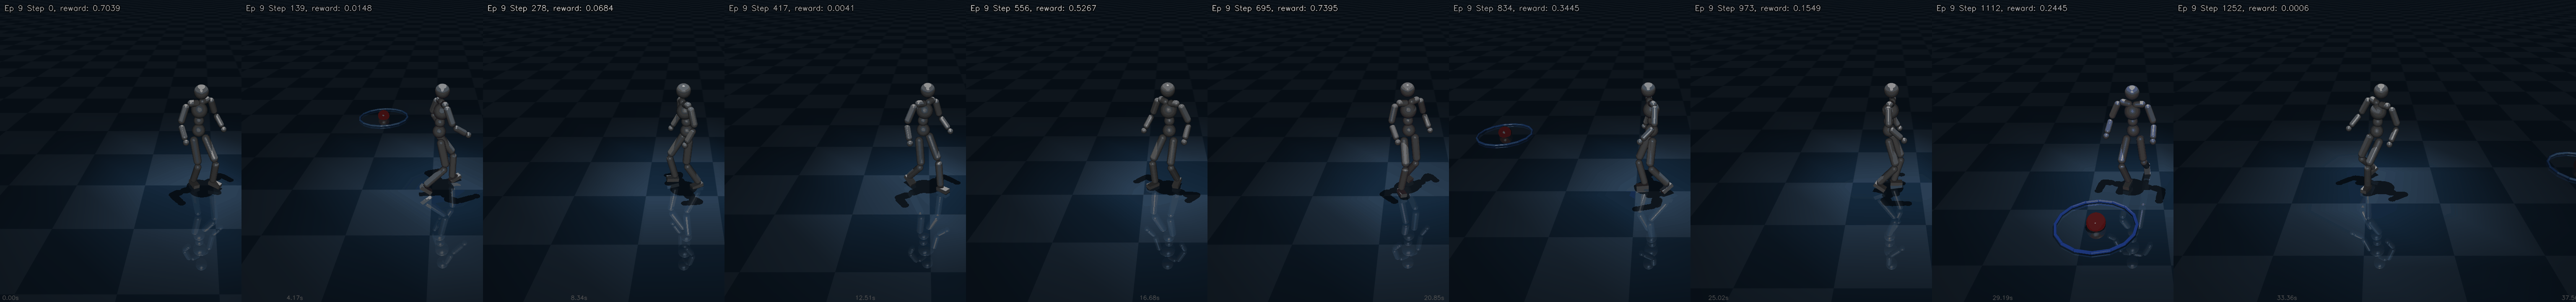
\includegraphics[width=\textwidth]{outputs/simulations/loco_walk.png}
    \caption{locomotion\_walk -- target-following with moderate turn capability}
    \label{fig:loco_walk_sim}
\end{figure}

\textbf{Walk.} Mimicry is acceptable across the diverse reference set, with the policy reliably orienting toward goals at small angular deviations. Lifetime 0.31 cycles, reward 0.163, and highest score\_fake (0.281) confirm strong imitation fidelity. Task reward (0.170) is highest among the three, indicating effective heading/location tracking. Wider angular deviations expose slower reorientation and weaker stability than crouch.

\begin{figure}[H]
    \centering
    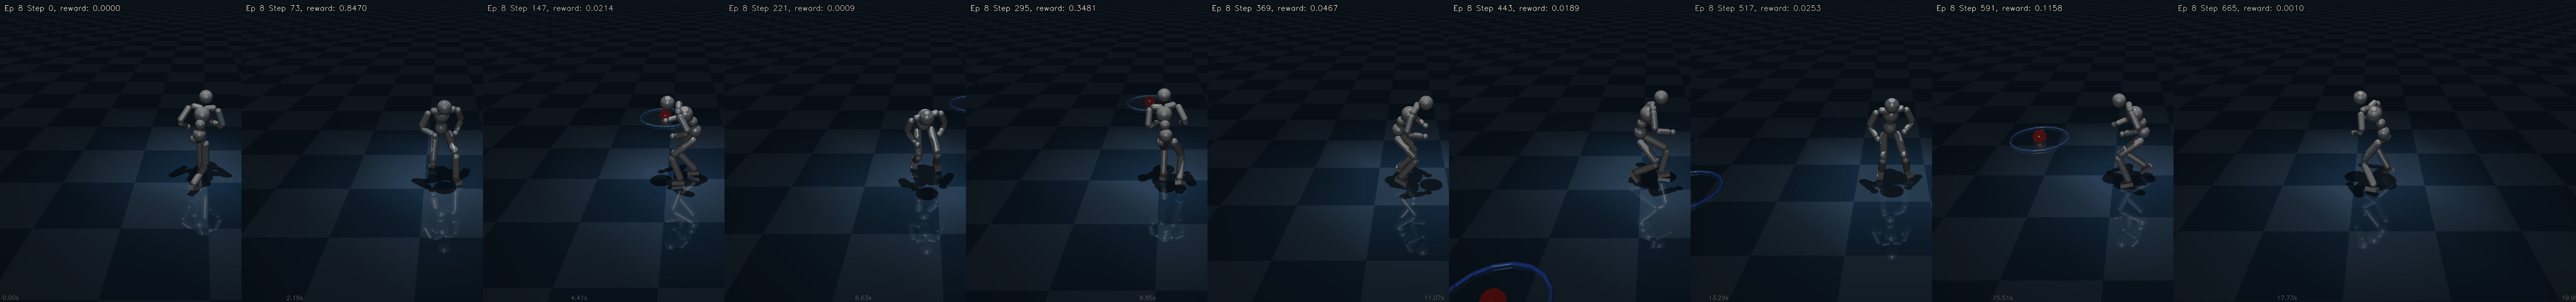
\includegraphics[width=\textwidth]{outputs/simulations/loco_crouch.png}
    \caption{locomotion\_crouch -- wide-deviation turns via stabilizing leg-drag gait}
    \label{fig:loco_crouch_sim}
\end{figure}

\textbf{Crouch.} Surprisingly strong task performance with longest survival (0.39 cycles) despite shortest training (666 steps). The controller turns toward wider goal deviations effectively. Inspection reveals an emergent stabilization hack: one leg moves slowly forward like a train-wheel while the other drags as support, preventing falls. This is reflected in elevated value-loss variance (0.14) and modest reward (0.064), signaling stable but non-textbook gait.

\begin{figure}[H]
    \centering
    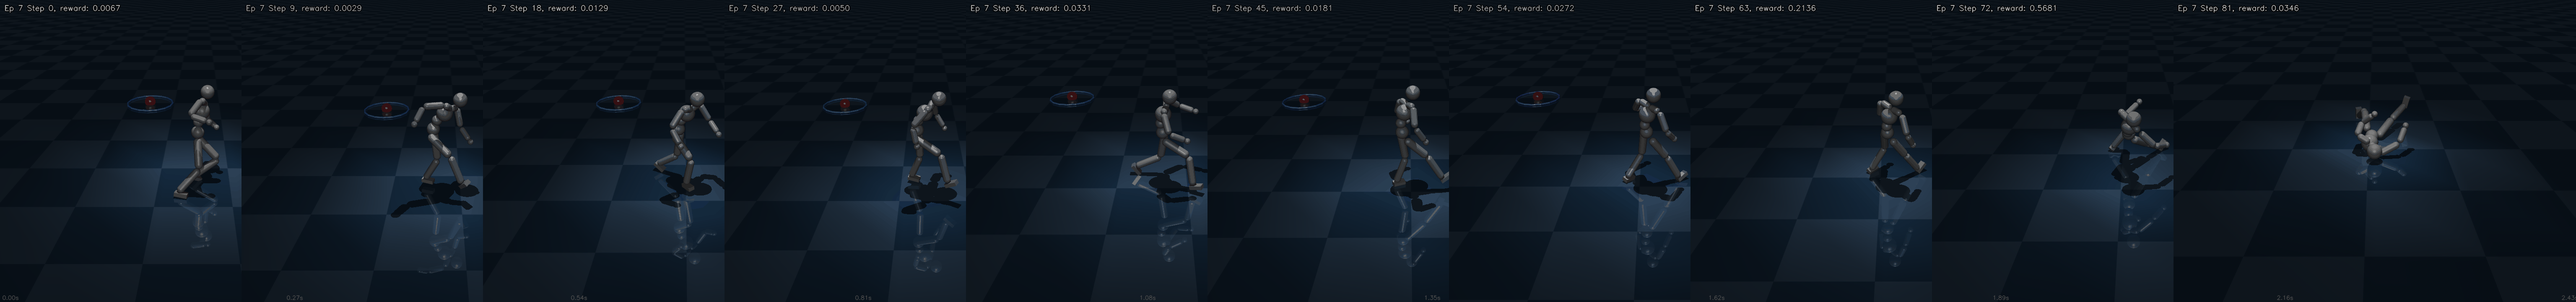
\includegraphics[width=\textwidth]{outputs/simulations/loco_run.png}
    \caption{locomotion\_run -- high-speed kangaroo hopping with stability failure}
    \label{fig:loco_run_sim}
\end{figure}

\textbf{Run.} High-speed dynamics overwhelm the policy: it adopts a kangaroo-like hopping gait, repeatedly skipping forward in attempts to stabilize before falling. Despite the longest training (2122 steps), lifetime collapses to 0.27 cycles with negative reward (-0.079) and lowest score\_fake (0.050)---less than partial imitation success. Task reward (0.078) is correspondingly low, confirming that mimicability remains the bottleneck before task completion can be evaluated reliably.

The task-based experiments demonstrate that goal-directed extensions integrate cleanly with the adversarial imitation backbone for low- and moderate-velocity gaits. High-velocity locomotion exposes the same DOF and momentum-transfer limitations identified in earlier categories, motivating the planned humanoid extension and richer discriminator window.
